\setmodule{7}

%BEGIN_FOLD % ====>>_____ Занятие 1 _____<<====
\begin{class}[number=1]
	\begin{listofex}
		\item Занятие 1
	\end{listofex}
\end{class}
%END_FOLD

%BEGIN_FOLD % ====>>_____ Занятие 2 _____<<====
\begin{class}[number=2]
	\begin{listofex}
		\item Занятие 2
	\end{listofex}
\end{class}
%END_FOLD

%BEGIN_FOLD % ====>>_ Домашняя работа 1 _<<====
\begin{homework}[number=1]
	\begin{listofex}
		\item В параллелограмме \(ABCD\): \(AB=4, AD=4, \sin A = 0,25 \).  Найдите большую высоту параллелограмма.
		\item Параллелограмм и прямоугольник имеют одинаковые стороны. Найдите острый угол параллелограмма, если его площадь равна половине площади прямоугольника. Ответ дайте в градусах.
		\item Стороны параллелограмма равны \(9\) и \(15\). Высота, опущенная на первую сторону, равна \(10\). Найдите высоту, опущенную на вторую сторону параллелограмма.
		\item Площадь параллелограмма равна \(40\), две его стороны равны \(5\) и \(10\). Найдите большую высоту этого параллелограмма.
		
		\item В треугольнике \(ABC\): \(AC=BC=27, AH\) --- высота, \(\sin BAC = \dfrac{ 2 }{ 3 }\). Найдите \(BH\).
		\item В треугольнике \(ABC\): \(AC = BC = 4\sqrt{15} \), \(\cos BAC = 0,25\). Найдите высоту \(AH\).
		\item Два угла треугольника равны \(58 \degree\) и \(72\degree \). Найдите тупой угол, который образуют высоты треугольника, выходящие из вершин этих углов. Ответ дайте в градусах.
		\item В треугольнике \(ABC\): \(CH\) --- высота, \(AD\) --- биссектриса, \(O\) --- точка пересечения прямых \(CH\) и \(AD\), \(\angle BAD = 26 \degree\). Найдите угол \(AOC\). Ответ дайте в градусах.
		\item Рабочие прокладывают тоннель длиной \(87\) метров, ежедневно увеличивая норму прокладки на одно и то же число метров. Известно, что за первый день рабочие проложили \(7\) метров туннеля. Определите, сколько метров туннеля проложили рабочие в последний день, если вся работа была выполнена за \(6\) дней.
		\item Бригада маляров красит забор длиной \(150\) метров, ежедневно увеличивая норму покраски на одно и то же число метров. Известно, что за первый и последний день в сумме бригада покрасила \(75\) метров забора. Определите, сколько дней бригада маляров красила весь забор.
		\item Теплоход проходит по течению реки до пункта назначения \(255\) км и после стоянки возвращается в пункт отправления. Найдите скорость теплохода в неподвижной воде, если скорость течения равна \(1\) км/ч, стоянка длится \(2\) часа, а в пункт отправления теплоход возвращается через \(34\) часа после отплытия из него. Ответ дайте в км/ч.
		\item Моторная лодка в \(10:00\) вышла из пункта \(A\) в пункт \(B\), расположенный в \(30\) км от \(A\). Пробыв в пункте \(B\) \(2\) часа \(30\) минут, лодка отправилась назад и вернулась в пункт \(A\) в \(18:00\). Определите (в км/ч) собственную скорость лодки, если известно, что скорость течения реки \(1\) км/ч.
	\end{listofex}
\end{homework}
%END_FOLD

%BEGIN_FOLD % ====>>_____ Занятие 3 _____<<====
\begin{class}[number=3]
	\begin{listofex}
		\item Занятие 3 
	\end{listofex}
\end{class}
%END_FOLD

%BEGIN_FOLD % ====>>_____ Занятие 4 _____<<====
\begin{class}[number=4]
	\begin{listofex}
		\item Занятие 4
	\end{listofex}
\end{class}
%END_FOLD

%BEGIN_FOLD % ====>>_ Домашняя работа 2 _<<====
\begin{homework}[number=2]
	\begin{listofex}
		\item
		\begin{minipage}[t]{\bodywidth}
			У треугольника со сторонами \(9\) и \(6\) проведены высоты к этим сторонам. Высота, проведенная к первой стороне, равна \(4\). Чему равна высота, проведенная ко второй стороне?
		\end{minipage}
		\hspace{0.02\linewidth}
		\begin{minipage}[t]{\picwidth}
			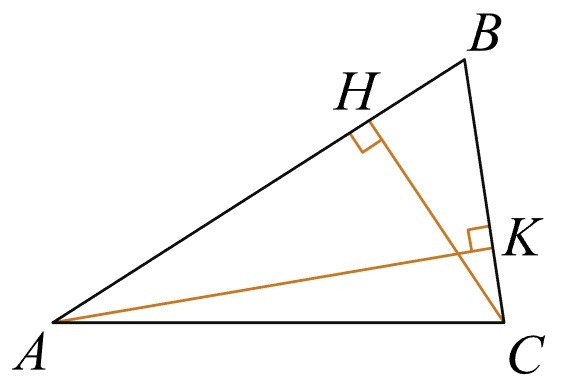
\includegraphics[align=t, width=\linewidth]{../\picpath/MECGERM9H2-1}
		\end{minipage}
		\item
		\begin{minipage}[t]{\bodywidth}
			В треугольнике \(ABC\) \(CH\) --- высота, \(AD\) --- биссектриса, \(O\) --- точка пересечения прямых \(CH\) и \(AD\), угол \(BAD\) равен \(26\degree \). Найдите угол \(AOC\). Ответ дайте в градусах.
		\end{minipage}
		\hspace{0.02\linewidth}
		\begin{minipage}[t]{\picwidth}
			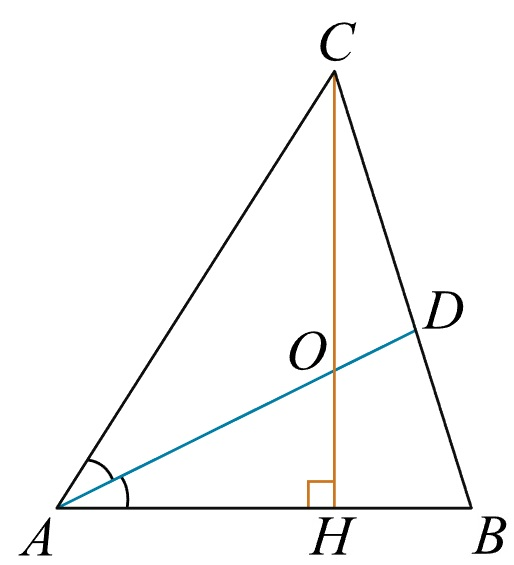
\includegraphics[align=t, width=\linewidth]{../\picpath/MECGERM9H2-2}
		\end{minipage}
		\item
		\begin{minipage}[t]{\bodywidth}
			В треугольнике \(ABC\) угол \(B\) равен \(45\degree \), угол \(C\) равен \(85\degree \), \(AD\) --- биссектриса, \(E\) --- такая точка на \(AB\), что \(AE  =  AC\). Найдите угол \(BDE\). Ответ дайте в градусах.
		\end{minipage}
		\hspace{0.02\linewidth}
		\begin{minipage}[t]{\picwidth}
			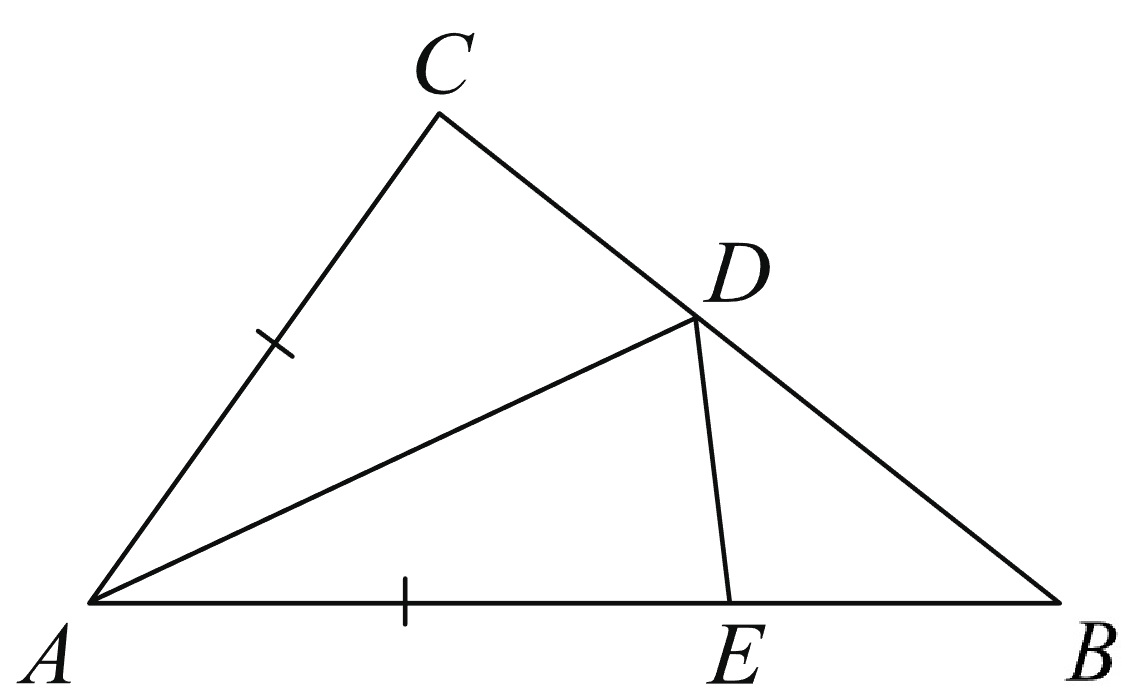
\includegraphics[align=t, width=\linewidth]{../\picpath/MECGERM9H2-3}
		\end{minipage}
		\item Диагональ прямоугольника вдвое больше одной из его сторон. Найдите больший из углов, который образует диагональ со сторонами прямоугольника? Ответ выразите в градусах.
		\item
		\begin{minipage}[t]{\bodywidth}
			Диагонали четырехугольника равны \(57\) и \(8\). Найдите периметр четырехугольника, вершинами которого являются середины сторон данного четырехугольника.
		\end{minipage}
		\hspace{0.02\linewidth}
		\begin{minipage}[t]{\picwidth}
			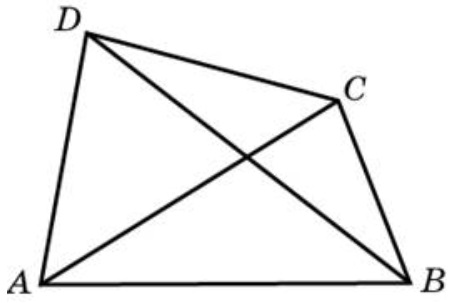
\includegraphics[align=t, width=\linewidth]{../\picpath/MECGERM9H2-4}
		\end{minipage}
		\item Площадь параллелограмма \(ABCD\) равна \(153\). Найдите площадь параллелограмма \(A'B'C'D'\), вершинами которого являются середины сторон данного параллелограмма.
		\item
		\begin{minipage}[t]{\bodywidth}
			Через концы \(A, B\) дуги окружности в \(62\degree \) проведены касательные \(AC\) и \(BC\). Найдите угол \(ACB\). Ответ дайте в градусах.
		\end{minipage}
		\hspace{0.02\linewidth}
		\begin{minipage}[t]{\picwidth}
			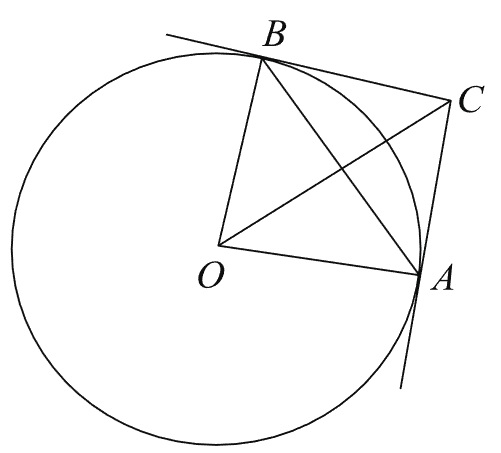
\includegraphics[align=t, width=\linewidth]{../\picpath/MECGERM9H2-5}
		\end{minipage}
		\item К окружности, вписанной в квадрат со стороной, равной \(a\), проведена касательная, пересекающая две его стороны. Найдите периметр отсеченного треугольника.
		\item Прямая касается окружности с центром \(O\) в точка \(A\). Точка \(C\) на этой прямой и точка \(D\) на окружности расположены по разные стороны от прямой \(OA\). Найдите угол \(CAD\), если угол \(AOD\) равен \(110 \degree\).
	\end{listofex}
\end{homework}
%END_FOLD

%BEGIN_FOLD % ====>>_____ Занятие 5 _____<<====
\begin{class}[number=5]
	\begin{listofex}
		\item Занятие 5
	\end{listofex}
\end{class}
%END_FOLD

%BEGIN_FOLD % ====>>_____ Занятие 6 _____<<====
\begin{class}[number=6]
	\begin{listofex}
		\item Занятие 6
	\end{listofex}
\end{class}
%END_FOLD

%BEGIN_FOLD % ====>>_ Домашняя работа 3 _<<====
\begin{homework}[number=3]
	\begin{listofex}
		\item Домашняя работа 3
	\end{listofex}
\end{homework}
%END_FOLD

%BEGIN_FOLD % ====>>_____ Занятие 7 _____<<====
\begin{class}[number=7]
	\title{Подготовка к проверочной}
	\begin{listofex}
		\item Занятие 7
	\end{listofex}
\end{class}
%END_FOLD

%BEGIN_FOLD % ====>>_ Проверочная работа _<<====
\begin{exam}
	\begin{listofex}
		\item Проверочная
	\end{listofex}
\end{exam}
%END_FOLD